\documentclass[11pt,a4paper]{article}
\usepackage[utf8]{inputenc}
\usepackage{amsmath}
\usepackage[margin=1.0in]{geometry}
\usepackage[pdftex]{graphicx}
\usepackage{amsfonts}
\usepackage{amssymb}
\usepackage{caption}
\usepackage{hyperref}
\hypersetup{
    colorlinks=true,
    citecolor=black,      
    urlcolor=cyan,
}
\usepackage[T1]{fontenc}
\renewcommand*{\figurename}{Rys.} 
\renewcommand*{\tablename}{Tab.} 
\author{Rafał Kornel}
\title{\textbf{Wzmacniacz operacyjny - badanie właściwości.}}
\date{}
\begin{document}
\maketitle

\section*{Abstrakt}
W doświadczeniu zbadano własności wzmacniacza operacyjnego o oznaczeniu uA741. Skonstruowano szereg układów niezbędnych do zbadania charakterystyk wzmacniacza. Udało się określić wzmocnienie wzmacniacza pracującego w trybie odwracającym fazę na 
$$ k = -10.11 \pm 0.11, $$
co zgadza się z wartością deklarowaną przez producenta. Rownież zbadano pasmo przenoszenia wzmacniacza, wynosi ono $[0, 10^4]$ Hz.  \\
Potwierdzono także właściwości całkujące urządzenia, określono pasmo dobrego całkowania na $[0.1, 1]$ kHz, a także różniczkujące, gdzie pasmo przenoszenia wyniosło $[5, 300]$ Hz.

\section*{Wstęp teoretyczny}
Wzmacniacz operacyjny jest elementem elektronicznym pełniący szereg funkcji. Ten układ scalony, przedstawiony na Rys.\ref{wzmacniacz1} odpowiednio podłączony do właściwego obwodu pełni role wzmacniacza. Poza wzmocnieniem sygnału wejściowego, może on odwrócić jego fazę, a także posłużyć jako element różniczkujący, bądź całkujący sygnał.
\begin{figure}[ht!]	
	\begin{center}
		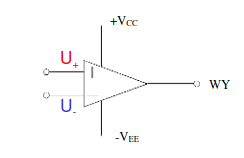
\includegraphics[width = 0.6\textwidth]{schemat_wzmacniacza.png}
		\caption{Symbol wzmacniacza operacyjnego, używany przy konstruowaniu obwodów wzmacniających. \cite{wzmacniacz}.}
		\label{wzmacniacz1}
	\end{center}
\end{figure}	
Na Rys.\ref{wzmacniacz1} zauważyć można, iż poza odnogą sygnału wyjściowego $WY$, wzmacniacz posiada dwie pary odnóg: $U_+$ / $U_-$, oraz $+V_{cc}$ \ $-V_{ee}$. Napięcie podane między odnogami $U_+$ oraz $U_-$ to nasz sygnał wejściowy, który chcemy wzmocnić. możemy jedną z odnóg podłączyć również do masy. Wtedy sygnał podany na $U_+$ (względem masy) będzie wzmacniany bez odwrócenia fazowego, zaś sygnał podany na $U_-$ (względem masy) będzie miał odwróconą fazę. Odnogi $+V_{cc}$ oraz $-V_{ee}$ służą do zasilienia układu, a zatem one dostarczą energii potrzebnej do wzmocnienia sygnału. W praktyce powinno się na każdą z odnóg podać prąd stały o ustalonwej wartości, lecz o przeciwnych znakach (zgodnie ze schematem).

\section*{Przebieg doświadczenia, uzyskane pomiary.}
W niniejszym doświadczeniu wykorzystano następujące przyrządy pomiarowe:
\begin{itemize}
\item{Generator funkcji Rigol DG1022}
\item{Zasilacz sieciowy Rigol DP832}
\item{Oscyloskop Rigol MSO1104z}
\item{Multimetr Rigol DM3058e}
\item{Lutownica}
\item{Płytka montażowa}
\end{itemize}
Krokiem "zerowym" było zmierzenie wartości oporów oraz pojemności otrzymanych elementów. Wartości te przedstawia Tab.\ref{opory}.

\begin{table}[!htp]
\begin{center}
\begin{tabular}{|c|c|}
\hline
$R_1$ & 5.6062 k$\Omega$ \\ \hline
$R_2$ & 56.553 k$\Omega$ \\ \hline
$R_3$ & 5.6025 k$\Omega$ \\ \hline
$R_4$ & 50.298 k$\Omega$ \\ \hline
$R_5$ & 5.1309 k$\Omega$ \\ \hline
$C$   & 95.3 nF          \\ \hline
\end{tabular}
\caption{Wartości oporów oraz pojemności użytych elementów.}
\label{opory}
\end{center}
\end{table}
Po rozpoznaniu oporników przystąpiono do skonstruowania układu wzmacniacza odwracającego, przestawionego na Rys.\ref{wzm_odwracajacy}. Napięcie zasilające jednak wzmacniacz zwiększono do +25V na odnodze $+V_{cc}$ oraz -25V na $-V_{ee}$.
Konsekwencje tej zmiany zostaną przedyskutowane w następnej sekcji. \\
Następnie zostały zebrane pomiary wartości $U_{wy}$ oraz $U_{we}$ dla punktów tej samej fazy, dla sygnału wejściowego o częstotliwości $f = 1000 \text{[Hz]}$. Dokonano tego za pomocą oscyloskopu wraz z funkcją kursorów. Wyniki przedstawia Tab.\ref{czesc1}. \\
Kolejnym krokiem było zebranie pomiarów maksymalnej wartości napięcia sygnału wejściowego $U_{we}$, oraz maksymalnej wartości napięcia sygnału wyjściowego $U_{wy}$ dla różnych wartości częstotliwości sygnału wejściowego $f$. Wyniki tej części zostały przedstawione w Tab.\ref{czesc2}. Pomiary zostały wykonane korzystając z wbudowanej funkcji oscyloskopu $V_{max}$. \\
Po zebraniu odpowiednich pomiarów został zmontowany układ realizujący funkcję całkowania sygnału wejściowego, a następnie układ różniczkujący sygnał. Schematy są przedstawione na Rys.\ref{wzm_calkujacy} oraz Rys.\ref{wzm_rozniczkujacy}.



\begin{figure}[ht!]	
	\begin{center}
		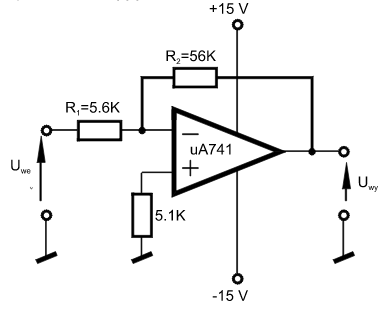
\includegraphics[width = 0.4\textwidth]{schemat_odwracajacy.png}
		\caption{Schemat układu realizującego wzmacniacz odwracający fazę. \cite{instrukcja}.}
		\label{wzm_odwracajacy}
	\end{center}
\end{figure}	

\begin{figure}[htp!]
\begin{minipage}{0.5\linewidth}

	\begin{center}
		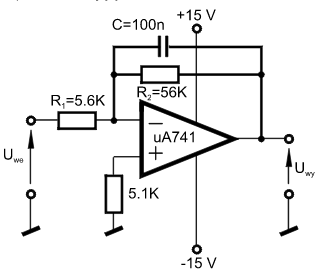
\includegraphics[width = 0.6\textwidth]{schemat_calkujacy.png}
		\caption{Schemat układu realizującego wzmacniacz całkujący sygnał. \cite{instrukcja}.}
		\label{wzm_calkujacy}
	\end{center}
\end{minipage}
\begin{minipage}{0.5\linewidth}
	\begin{center}
		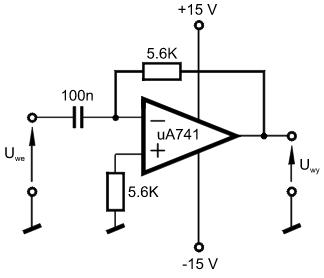
\includegraphics[width = 0.6\textwidth]{schemat_rozniczkujacy.png}
		\caption{Schemat układu realizującego wzmacniacz różniczkujący sygnał. \cite{instrukcja}.}
		\label{wzm_rozniczkujacy}
	\end{center}
\end{minipage}
\end{figure}

\begin{table}[!htp]
\begin{minipage}{.4\linewidth}
\begin{center}
\begin{tabular}{|c|c|}
\hline
\multicolumn{1}{|l|}{$U_{we}$ {[}V{]}} & \multicolumn{1}{l|}{$U_{wy} [V]$} \\ \hline
0.3                                    & -2.8                              \\
0.74                                   & -7.0                                \\
0.86                                   & -8.4                              \\
1.06                                   & -10.4                             \\
1.24                                   & -12.4                             \\
1.44                                   & -14.2                             \\
1.61                                   & -16.0                               \\
1.75                                   & -17.4                             \\
1.87                                   & -18.8                             \\
2.0                                      & -20.0                               \\
1.85                                   & -18.0                               \\
1.45                                   & -14.4                             \\
\hline
\end{tabular}
\caption{Pomiary części pierwszej doświadczenia, służące do wyznaczenia zależności wzmocnienia wzmacniacza dla ustalonej częstotliwości.}
\label{czesc1} 
\end{center}
\end{minipage}
\begin{minipage}{.6\linewidth}
\begin{center}
\begin{tabular}{|r|c|c|}
\hline
\multicolumn{1}{|l|}{$f [Hz]$} & \multicolumn{1}{l|}{$U_{we} [mV]$} & \multicolumn{1}{l|}{$U_{wy} [V]$} \\ \hline
10                             & 512                                & 5.12                              \\
20                             & 512                                & 5.12                              \\
40                             & 512                                & 5.12                              \\
100                            & 512                                & 5.12                              \\
200                            & 512                                & 5.12                              \\
400                            & 512                                & 5.12                              \\
1000                           & 512                                & 5.12                              \\
2000                           & 512                                & 5.12                              \\
4000                           & 512                                & 5.12                              \\
10000                          & 512                                & 5.12                              \\
20000                          & 512                                & 5.04                              \\
40000                          & 512                                & 4.72                              \\
100000                         & 512                                & 2.16                              \\
200000                         & 512                                & 0.96                              \\
400000                         & 512                                & 0.32                              \\
1000000                        & 512                                & 0.00 
\\
2000000                        & 512                                & 0.00                                
\\
\hline
\end{tabular}
\caption{Pomiary części drugiej doświadczenia, służące do wyznaczenia zależności wzmocnienia od częstotliwości sygnału wejściowego.}
\label{czesc2}
\end{center}
\end{minipage}

\end{table}

\section*{Analiza danych}
\subsection*{Wzmacniacz odwracający}
W pierwszej części doświadczenia zostały zmierzone wartości napięcia wyjściowego jako funkcji napięcia wejściowego dla sygnału wejściowego o częstotliwości $f=1000$ [Hz], $U_{wy} (U_{we})$. Spodziewamy się zależności liniowej o współczynniku proporcjonalności $k$:
$$ U_{wy} = k \cdot U_{we} + b. $$
 \begin{figure}[ht!]	
	\begin{center}
		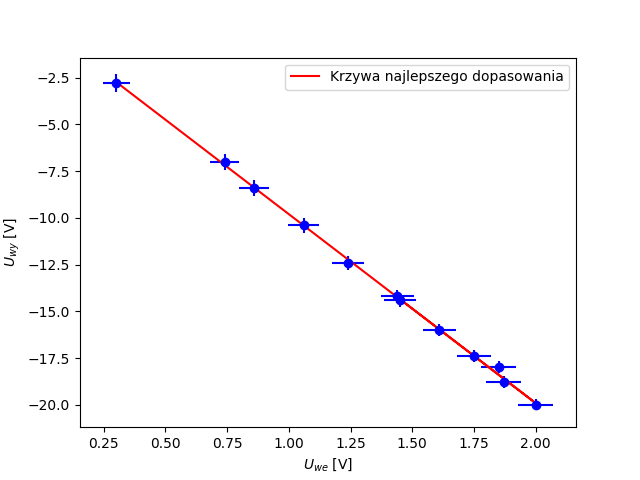
\includegraphics[width = 0.6\textwidth]{Figure_1.png}
		\caption{Pomiary napięcia wyjściowego w funkcji napięcia wejściowego, wraz z dopasowaniem liniowym.}
		\label{wykres1}
	\end{center}
\end{figure}	
Taka zależność została dopasowana do pomiarów, co przedstawia Rys.\ref{wykres1}. Niepewności zostały policzone według następującego wzoru:
$$ \delta_{U} = M \cdot 0.1 + U \cdot 0.01 + 0.002 \text{[V]},$$
gdzie $M$ to podziałka oscyloskopu użyta podczas wykonywania pomiarów, która wynosiła odpowiednio
$$ M_{U_{we}} = 0.5 \text{V}, \qquad M_{U_{wy}} = 5 \text{V} $$
dla pomiarów z Tab.\ref{czesc1}, oraz 
$$ M_{U_{we}} = 0.2 \text{V}, \qquad M_{U_{wy}} = 2 \text{V} $$
dla pomiarów z Tab.\ref{czesc2}. Uznajemy, że częstotliwość sygnału wejściowego znamy dokładnie.
Dopasowanie zostało wykonane przy użyciu biblioteki $scipy$ w języku $python$. W rezultacie otrzymano:
$$ k = -10.11 \pm 0.11 \qquad b = 0.30 \pm 0.17 \text{[V]}. $$
Porównując do wartości wynikającej ze specyfikacji wzmacniacza, $k_s = -10$ widzimy bardzo niewielką różnicę, ponadto wartość dokładna mieści się w przedziale $[k - \mu_k, k + \mu_k]$. Współczynnik $b$ powinien być równy 0, nie zawiera się on zatem w przedziale $[b - \mu_b, b + \mu_b]$. Celem doświadczenia było wyznaczenie zakresu liniowości wzmacniacza dla częstotliwości $f = 1000$ [Hz]. Wcześniej wspomniano, iż napięcie zasilające wzmacniacz zostało zmienione do do $\pm 25$ [V]. Spowodowało to, że zakres liniowości uległ zmianie, tak, że cały zawiera się w zakresie w którym wykonano pomiary. Można więc orzec, że dla napięć z zakresu [0.3, 2.0] Volta wzmacniacz pracuje liniowo. \\ \\
W drugiej części doświadczenia zbadana została zależność wzmocnienia od częstotliwości sygnału wejściowego. 
Wzmocnienie zostało policzone według wzoru:
$$ k = \frac{U_{wy}}{U_{we}}. $$
 \begin{figure}[ht!]	
	\begin{center}
		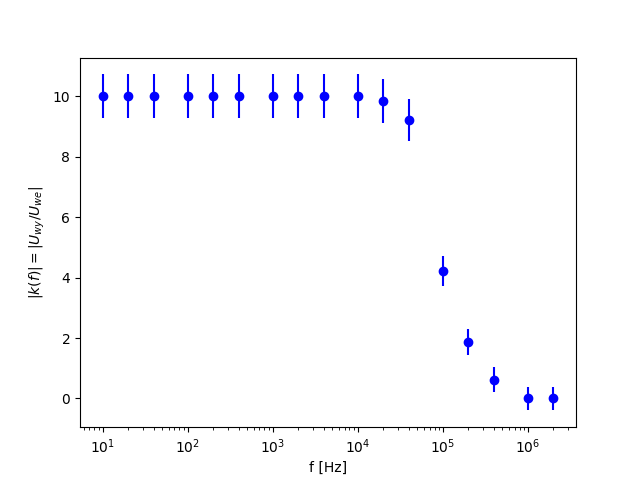
\includegraphics[width = 0.6\textwidth]{Figure_2.png}
		\caption{Zależność wzmocnienia $k$ od częstotliwości sygnału wejściowego.}
		\label{wykres2}
	\end{center}
\end{figure}	
Niepewność wzmocnienia została policzona korzystając z metody propagacji małych błędów:
$$ \mu_k = [ (\frac{\mu_{U_{wy}}}{U_{we}})^2 + ( \frac{U_{wy}\cdot \mu_{U_{we}}}{U_{we}^2} )^2 ]^{\frac{1}{2}}.$$ \\
Widać na Rys.\ref{wykres2}, iż wzmacniacz dla częstotliwości z zakresu $[0, 10^4]$ ma moduł wzmocnienia bardzo zbliżony do $|k|=10$, wynikającego ze specyfikacji układu. Możemy zatem orzec, iż jest to pasmo przenoszenia badanego wzmacniacza.

\subsection*{Wzmacniacz całkujący}
Po zbadaniu charakterystyki wzmacniacza odwracającego fazę, zbadano własności wzmacniacza całkującego. Realizuje go układ widoczny na Rys.\ref{wzm_calkujacy}. Dla częstotliwości sygnału wejściowego rzędu 1 - 10 Hz o kształcie prostokątnym sygnał był wzmacniany ze współczynnikiem $k \sim. 10.$ Ustalono amplitudę sygnału wejściowego na 1 V. Przy zwiększaniu częstotliwości sygnał deformował się, aż przy $f \sim 100$ Hz zaczął przypominać sygnał piłokształtny. Dalej sygnał był dobrze całkowalny, aż do częstotliwości $f \sim 100$ kHz, po czym zaczął wykazywać zachowanie typu $sin(\omega_1 t) \cdot e^{-\omega_2 t}$, podobne do wariacji funkcji przy nieciągłościach podczas kompozycji funkcji prostokątnej z okresowych funkcji poprzez szereg (skończony) Fouriera. Można podsumować, iż wzmacniacz dobrze całkował sygnał dla zakresu $[0.1, 100]$ kHz.

\subsection*{Wzmacniacz różniczkujący}
Następnie zmontowano układ realizujący różniczkowanie sygnału wejściowego, przedstawiony na Rys.\ref{wzm_rozniczkujacy}.  Rozpoczęto od ustalenia sygnału wejściowego o kształcie piłokształtnym z amplitudą 100 mV oraz częstotliwością 100 Hz. Na wyjściu zauważono sygnał prostokątny, dla częstotliwości sięgających do $ f \sim 300$ Hz. Powyżej tych częstotliwości występowało zjawisko takie jak przy wzmacniaczu całkującym dla wysokich częstotliwości. Dolną granicą dobrego różniczkowania sygnały była częstotliwość $f \sim 5$ Hz. Poniżej tej częstotliwości sygnał wyjściowy był bardzo słaby, jego amplituda sięgała rzędu 10 mV. Nie dało się odróżnić go od szumu. Podsumowując, zakres dobrego różniczkowania tego układu wynosił $[5, 300]$ Hz.

\section*{Podsumowanie}
Otrzymane wartości wzmocnienia są bardzo dobrze zgodne z wartością podaną przez producenta. Zakres liniowości wzmacniacza zaś, został prawdopodobnie zwiększony poprzez zmianę napięcia zasilania, co skutkowało uzyskaniem tylko liniowych pomiarów, w możliwym do zmierzenia zakresie napięć wejściowych. Podczas ponownego wykonania eksperymentu należy nie przejmować się, iż sygnał (przy podaniu napięcia zasilania $\pm 15$V jest w pewnym momencie ucięty. Jest to oczekiwany efekt. \\
Poprawnie także zbadano własności różniczkujące i całkujące wzmacniacza. Udało się wyznaczyć przedział dobrego różniczkowania oraz całkowania.


\begin{thebibliography}{}
	\bibitem{wzmacniacz} Rysunek schematyczny pochodzący z wykładu Pracowni elektronicznej dla astronomów.
	\bibitem{instrukcja} Schematy pochodzą z instrukcji doświadczenia http://pracownie1.fuw.edu.pl/pe-A/pliki/Instr\_Wzmacniacz\_2016.pdf
	\bibitem{niepewnosci} Specyfikacja oscyloskopu Rigol DS1000Z-E https://www.batronix.com/files/Rigol/Oszilloskope/DS1000Z-E/DS1000Z-E-Data-sheet.pdf
\end{thebibliography}

\end{document}